\section{Particle interactions and thermal production}\label{sec:thermal}

\subsection{A neutral scalar and the scattering amplitude}\label{sec:scalar-scattering}
For a concrete collider and direct-detection test, let $S$ denote a stable real $Z_2$-odd scalar. This section specifies an additional effective particle model, with its own mass and coupling inputs. Particle amplitudes use signature $(+,-,-,-)$, $p^2=E^2-\mathbf p^2$, and $\hbar=c=1$ unless units are restored explicitly. This convention and the gravitational signature in Section~\ref{sec:metric} describe the same physical invariants after the corresponding metric-sign change. Consider
\begin{equation}
\mathcal L_S=\frac12(\partial_\mu S)^2-\frac12m_0^2S^2-\frac{\lambda_S}{4}S^4
-\frac{\lambda_{HS}}2S^2H^\dagger H,\qquad
m_S^2=m_0^2+\frac{\lambda_{HS}v^2}{2}.
\end{equation}
At low momentum transfer, Higgs exchange gives the leading tree-level spin-independent nucleon cross section
\begin{equation}\label{eq:si}
\sigma_{\rm SI}=\frac{\lambda_{HS}^2f_N^2\mu_{SN}^2m_N^2}{4\pi m_h^4m_S^2}
\times(\hbar c)^2,
\quad \mu_{SN}=\frac{m_Sm_N}{m_S+m_N},
\end{equation}
where particle masses and the first factor are expressed in natural units and the final factor converts to physical area. The scalar nucleon form factor $f_N$ carries a significant hadronic uncertainty and must be propagated in a physical fit. We use $m_h=125.1$ GeV, $m_N=0.939$ GeV, and $f_N=0.30$ solely as benchmark inputs.

For $m_S=40$ GeV and $\lambda_{HS}=0.01$, Eq.~\eqref{eq:si} yields
\begin{equation}
\boxed{\sigma_{\rm SI}(40\,\Gev)=5.282\times10^{-46}\ \mathrm{cm}^2.}
\end{equation}
The 2025 LUX--ZEPLIN combined-exposure result gives a 90\% confidence upper limit of $2.2\times10^{-48}\,\mathrm{cm}^2$ at $40$ GeV \cite{LZ25}. For comparison, the XENONnT 3.1 tonne-year analysis reports a 90\% minimum of $1.7\times10^{-47}\,\mathrm{cm}^2$ at $30$ GeV; the comparison at $40$ GeV uses the exclusion curve evaluated at that mass \cite{XENON25}. The 40-GeV illustrative point is about $240$ times the LZ limit at that mass and is excluded under the standard elastic nuclear-recoil assumptions. The exclusion concerns this selected effective-theory point and the assumed local scalar abundance. The published limit is a spin-independent elastic-scattering constraint for the adopted local-halo model \cite{LZ25}.

For the separate illustrative parameter choice $m_S=300$ GeV, $\lambda_{HS}=0.20$, Eq.~\eqref{eq:si} gives $3.910\times10^{-45}$ cm$^2$. Its experimental comparison is defined by the exclusion curve at $300$ GeV, the detector response and the local scalar fraction.

\subsection{The partial Higgs-pair contact rate}\label{sec:contact-rate}
The $S^2h^2$ contact vertex produces a partial annihilation rate
\begin{equation}
\left.\sigv\right|_{SS\to hh,\,\rm contact}
=\frac{\lambda_{HS}^2}{64\pi m_S^2}\sqrt{1-\frac{m_h^2}{m_S^2}},\qquad m_S>m_h.
\end{equation}
At $m_S=300$ GeV and $\lambda_{HS}=0.20$ this is $2.345\times10^{-26}$ cm$^3$ s$^{-1}$. Substitution into the frequently used thermal scaling $\Om_Sh^2\simeq0.12(2.2\times10^{-26}\,\mathrm{cm^3\,s^{-1}}/\sigv)$ gives $0.113$ \emph{for this partial-channel scaling estimate}. This partial-channel scaling isolates the contact contribution. The full tree-level two-body benchmark in Sec.~\ref{sec:portal-complete} includes interference, gauge and fermion final states, thresholds and thermal averaging. The abundance equation is
\begin{equation}
\frac{\dd Y}{\dd x}=-\frac{s(T)\sigv_{\rm full}(T)}{H(T)x}\bigl(Y^2-Y_{\rm eq}^2\bigr),\qquad x=m_S/T,
\end{equation}
for constant entropy degrees of freedom. With varying $g_{*s}$, entropy conservation supplies the factor $\mathcal A_s(T)$ derived below. The contact-only rate defines the limiting constant-rate equation below.

\subsection{Decay-driven freeze-in from an equilibrated parent}\label{sec:decay-freezein}
A distinct production model assumes a thermal scalar parent $A$ with mass $M_A$, one internal degree of freedom, and a feebly coupled stable daughter $S$. The parent undergoes $A\to S\varphi$, where $\varphi$ is a light bath particle, with partial width $\Gamma_A$. The exact parity assignment makes $A$ and $S$ odd and $\varphi$ even. The specified model takes $S$ to be the lightest odd particle and imposes $M_A>m_S+m_\varphi$; the allowed parent decay then preserves the daughter's parity protection. The model assumes bath interactions that equilibrate $A$ and a feeble daughter-production sector. For radiation domination, Maxwell--Boltzmann statistics, approximately constant entropy and energy degrees of freedom $g_{*s},g_{*\rho}$, and negligible inverse reactions,
\begin{align}
\gamma_{A\to S\varphi}&=\frac{g_A\Gamma_A M_A^2 T}{2\pi^2}K_1(M_A/T),\\
\frac{\dd Y_S}{\dd x}&=\frac{45g_A\Gamma_AM_{\rm Pl}}{4\pi^4\,1.66\,g_{*s}\sqrt{g_{*\rho}}\,M_A^2}
\,x^3K_1(x),\quad x=M_A/T.\label{eq:fimain}
\end{align}
The decay produces exactly one $S$ per event, so the source term and integrated yield have the normalization
\begin{equation}\label{eq:fi}
\boxed{Y_S(\infty)=\frac{135\,g_A\,\Gamma_AM_{\rm Pl}}
{8\pi^3\,1.66\,g_{*s}\sqrt{g_{*\rho}}\,M_A^2},}
\end{equation}
since $\int_0^\infty x^3K_1(x)\dd x=3\pi/2$. The number of dark particles per decay is fixed by the stated $A\to S\varphi$ channel. For a parent producing two $S$ particles, Eq.~\eqref{eq:fi} would acquire an additional factor of two. The equilibrium parent assumption specifies a bath-coupled parent whose thermalizing reactions are distinct from the feeble daughter-production channel.

Using $M_A=1000$ GeV, $m_S=10$ GeV, $g_{*s}=g_{*\rho}=106.75$, and a physical one-daughter decay width of $10^{-20}$ GeV gives
\begin{equation}
Y_S(\infty)=3.6292\times10^{-11},\qquad
\Om_Sh^2=2.742\times10^8\left(\frac{m_S}{\Gev}\right)Y_S
=\boxed{0.09951}.
\end{equation}
The rate-to-expansion ratio at $T=M_A$ is $\Gamma_A/H\simeq7.12\times10^{-9}$. This small ratio is a diagnostic of the specified feeble decay source. The calculation assumes that the stated decay dominates daughter production and that daughter thermalization is negligible. Adaptive quadrature of Eq.~\eqref{eq:fimain} from $x=10^{-3}$ gives the final-to-analytic ratio $0.9999999999293$, consistent with the finite-temperature estimate in Sec.~\ref{sec:finite-reheating}. The model uses constant $g_*$, instantaneous reheating, Maxwell--Boltzmann statistics and the single decay channel. Its masses and width are independent effective-model inputs. The limiting yield scales as $Y_\infty\propto \Gamma_A M_{\rm Pl}/(g_{*s}\sqrt{g_{*\rho}}M_A^2)$, so its logarithmic sensitivities are $\partial\ln Y/\partial\ln\Gamma_A=1$, $\partial\ln Y/\partial\ln M_A=-2$, $\partial\ln Y/\partial\ln g_{*s}=-1$, and $\partial\ln Y/\partial\ln g_{*\rho}=-1/2$. These derivatives propagate a specified parameter covariance into the yield covariance.

\begin{figure}[t]
\centering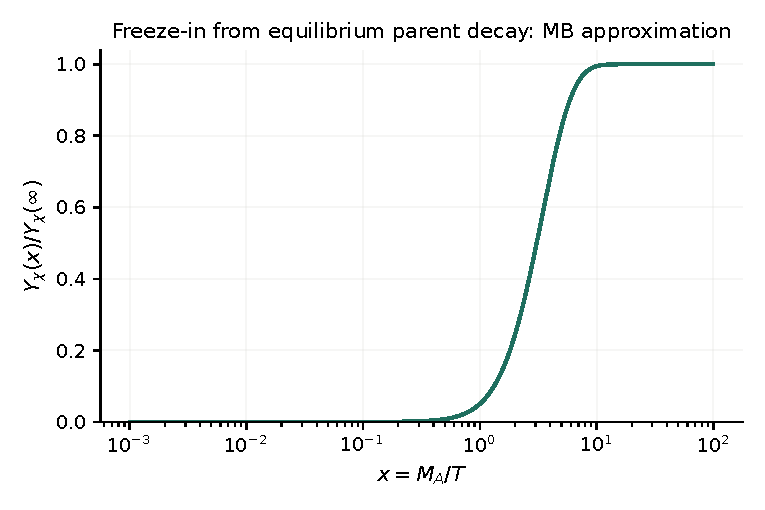
\includegraphics[width=.79\linewidth]{figures/freezein_yield.pdf}
\caption{Accumulated freeze-in yield in the explicit Maxwell--Boltzmann decay-source benchmark. The curve is normalized to its analytic asymptotic yield.}
\end{figure}

\subsection{Indirect-detection observables}
For the self-conjugate scalar $S$, annihilation produces a gamma-ray flux from a target with line-of-sight density factor $J$,
\begin{equation}
\frac{\dd\Phi_\gamma}{\dd E}=\frac{\sigv}{8\pi m_S^2}\frac{\dd N_\gamma}{\dd E}\,J,\qquad
J=\int_{\Delta\Om}\dd\Om\int \rho_S^2\,\dd\ell.
\end{equation}
For a specified final state, the Fermi--LAT likelihood combines the photon spectrum, branching fractions, density-squared $J$ factors and instrument response. The 14- and approximately 17-year dwarf-spheroidal analyses give bounds on the annihilation contribution \cite{Fermi24,Fermi26}. Antiproton inference additionally includes Galactic propagation, nuclear production and solar modulation \cite{AMS24}. These observables test the annihilation kernel of a specified candidate; the decay-only freeze-in example defines its production history through a separate collision term.

\subsection{Laboratory and abundance inversions}

For the selected scalar Higgs-portal normalization, the zero-momentum spin-independent cross section is quadratic in $\lambda_{HS}$, with other parameters held fixed. The original $m_S=40$ GeV, $\lambda_{HS}=0.01$ reference gives $\sigma^{\rm SI}_N=5.2815843\times10^{-46}$ cm$^2$. The LZ 4.2 tonne-year combined limit at this mass is $\sigma^{\rm SI}_{N,90}=2.2\times10^{-48}$ cm$^2$ \cite{LZ25}. Algebraic inversion, with the same halo model and nuclear conventions as the published limit, yields
\begin{equation}\label{eq:portalbound}
\boxed{|\lambda_{HS}|\leq 0.01\sqrt{\frac{2.2\times10^{-48}}{5.2815843\times10^{-46}}}=6.4540\times10^{-4}},\qquad
\frac{\sigma_N^{\rm SI}(0.01)}{\sigma_{N,90}^{\rm SI}}=240.07.
\end{equation}
This is a bound on the chosen low-energy portal model; its interpretation assumes that the candidate constitutes all of the local halo and scatters elastically and spin-independently. For a local fraction $0<f_{\rm loc}\leq1$ and the same velocity distribution, the rate constrains $f_{\rm loc}\sigma_{\rm SI}$ and the coupling bound scales as $f_{\rm loc}^{-1/2}$.  For a source-defined QICT candidate, the matched nucleon vertex supplies the amplitude in the same detector-response functional.

For one dark daughter per thermal parent decay, Eq.~\eqref{eq:fi} makes the asymptotic abundance linear in the partial decay width. Inverting the earlier reference scenario against the measured $\Omega_ch^2\simeq0.120$ \cite{Planck} yields
\begin{equation}\label{eq:widthinv}
\boxed{\Gamma_A^{\rm required}=1.205877\times10^{-20}\ \Gev,\qquad
\left.\frac{\Gamma_A}{H}\right|_{T=M_A}=8.58396\times10^{-9}.}
\end{equation}
Equation~\eqref{eq:widthinv} gives the decay width selected by the observed abundance within this effective production model.

\subsection{The constant-rate Boltzmann equation}
\label{sec:constant-freezeout}
A separate, specified freeze-out test evolves the comoving abundance with constant entropy/energy degrees of freedom, Maxwell--Boltzmann equilibrium and constant $s$-wave annihilation rate:
\begin{align}
\frac{\dd Y}{\dd x}&=-\frac{s\langle\sigma v\rangle}{Hx}(Y^2-Y_{\rm eq}^2),\qquad
Y_{\rm eq}=\frac{45g_\chi}{4\pi^4g_{*s}}x^2K_2(x),\\
\frac{s\langle\sigma v\rangle}{Hx}&=\frac{2\pi^2}{45\cdot1.66}\frac{g_{*s}}{\sqrt{g_{*\rho}}}\frac{M_{\rm Pl}m_\chi\langle\sigma v\rangle}{x^2}.
\end{align}
Numerical integration using $m_\chi=300$ GeV, $g_\chi=1$, $g_{*s}=g_{*\rho}=90$, and the previously stated contact-only reference rate $\langle\sigma v\rangle=2.345311\times10^{-26}$ cm$^3$s$^{-1}$, starting at $x=8$ in equilibrium, gives
\begin{equation}\label{eq:freezeoutfull}
\boxed{Y_\infty=1.219574\times10^{-12},\qquad
\Omega_\chi h^2=0.100322.}
\end{equation}
The integration uses a scaled abundance and an analytic late-time tail. An independent endpoint-and-step study is recorded in the numerical convergence data. This solves the specified constant-rate limiting Boltzmann equation. It is distinct from the thermally averaged portal calculation in Sec.~\ref{sec:portal-complete}, whose complete tree-level two-body amplitude supplies the physical annihilation rate within that benchmark.

\begin{figure}[t]\centering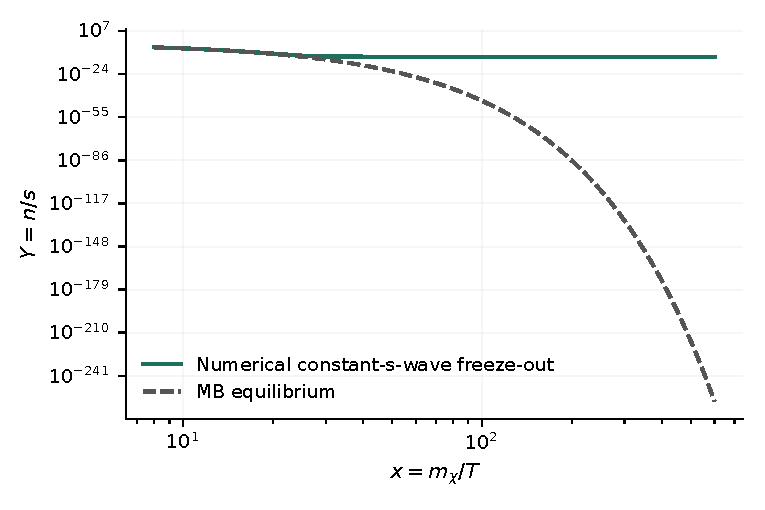
\includegraphics[width=.78\linewidth]{figures/freezeout_toy_exact_ode.pdf}\caption{Numerical solution of the fixed-rate single-species Boltzmann equation, with its Maxwell--Boltzmann equilibrium distribution. All masses and rates are external benchmark parameters.}\end{figure}

\subsection{Thermally averaged two-body Higgs-portal calculation}\label{sec:portal-complete}
The stated scalar interaction also determines a more complete, independently reproducible tree-level benchmark. With $\lambda=\lambda_{HS}$ and $v=246.22$ GeV, the Higgs-pair amplitude includes the contact, $s$-channel and both scalar-exchange diagrams:
\begin{equation}\label{eq:hh-amplitude}
\mathcal M_{hh}=-\lambda\left[1+\frac{3m_h^2}{s-m_h^2+im_h\Gamma_h}
+\lambda v^2\left(\frac1{t-m_S^2}+\frac1{u-m_S^2}\right)\right].
\end{equation}
The overall phase is immaterial. The symmetry factor for identical final Higgs particles gives
\begin{equation}
(\sigma v_{\rm M})_{hh}=\frac{\sqrt{1-4m_h^2/s}}{32\pi s}
\int_{-1}^{1}|\mathcal M_{hh}|^2\,\dd\cos\vartheta.
\end{equation}
Here $v_{\rm M}=2\sqrt{1-4m_S^2/s}$ in the centre-of-mass frame. Other open two-body channels are determined by the tree-level width of a virtual Higgs of invariant mass $\sqrt s$ \cite{Cline13}:
\begin{align}
(\sigma v_{\rm M})_{\rm SM\setminus hh}
&=\frac{2\lambda^2v^2\Gamma^{\rm tree}_{h\to WW,ZZ,f\bar f}(\sqrt s)}
{\sqrt s[(s-m_h^2)^2+m_h^2\Gamma_h^2]},\\
\Gamma_{f\bar f}(\sqrt s)&=\frac{N_c m_f^2\sqrt s}{8\pi v^2}
\left(1-\frac{4m_f^2}{s}\right)^{3/2},\\
\Gamma_{WW}(\sqrt s)&=\frac{s^{3/2}}{16\pi v^2}\sqrt{1-4r_W}
(1-4r_W+12r_W^2),\qquad r_V=m_V^2/s,
\end{align}
and $\Gamma_{ZZ}$ has the corresponding $1/(32\pi v^2)$ coefficient. Each contribution is included above its threshold. We use the vacuum input masses and fixed Yukawa representatives listed in the code; the propagator width is $\Gamma_h=4.07$ MeV. This defines a tree-level two-body benchmark with constant $g_{*s}=g_{*\rho}=90$. Quantum corrections, running couplings and thermal self-energies define additional physical refinements.

Maxwell--Boltzmann kinetic equilibrium gives the relativistic thermal average \cite{Gondolo91}
\begin{equation}\label{eq:thermal-average}
\langle\sigma v\rangle_T=\frac1{8m_S^4TK_2^2(m_S/T)}
\int_{4m_S^2}^{\infty}\sigma(s)(s-4m_S^2)\sqrt s\,K_1(\sqrt s/T)\,\dd s.
\end{equation}
Scaled Bessel functions and Gaussian quadrature evaluate this expression without exponential underflow. For the selected $m_S=300$ GeV, $\lambda=0.20$ point,
\begin{equation}\label{eq:portal-results}
\boxed{\begin{aligned}
(\sigma v)_{T\to0}&=1.13490\times10^{-25}\ \mathrm{cm^3\,s^{-1}},\\
\langle\sigma v\rangle_{x=20}&=9.78460\times10^{-26}\ \mathrm{cm^3\,s^{-1}},\\
Y_\infty&=2.85098\times10^{-13},\qquad \Omega_Sh^2=0.0234522.
\end{aligned}}
\end{equation}
The abundance is obtained by integrating the Boltzmann equation with the thermal rate and its post-endpoint annihilation tail. It is a conditional prediction of this specified Higgs-portal benchmark. The selected point supplies about $19.54\%$ of the reference $\Omega_ch^2=0.120$ through this thermal history; its direct-detection rate scales with the actual local scalar fraction. The contact-only calculation in Eq.~\eqref{eq:freezeoutfull} isolates a distinct limiting collision kernel.

\begin{figure}[htbp]\centering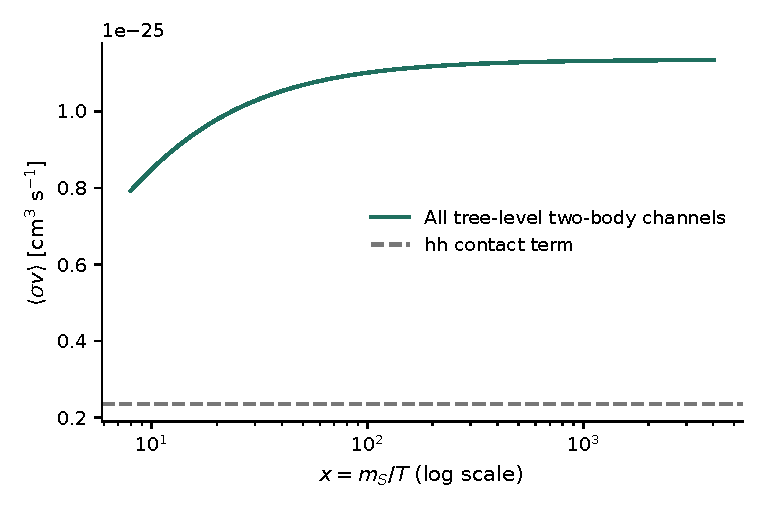
\includegraphics[width=.8\linewidth]{figures/portal_thermal_rates.pdf}
\caption{Thermally averaged annihilation into all tree-level two-body final states at the selected 300-GeV scalar point. The dashed line is the Higgs-pair contact contribution. Fixed vacuum parameters and constant relativistic degrees of freedom define the calculation.}\end{figure}

\subsection{The asymptotic tail of the constant-rate limiting equation}
For a constant annihilation coefficient $K$, the late equation is $Y'=-KY^2/x^2$ once $Y_{\rm eq}$ is exponentially small. Integration gives
\begin{equation}\label{eq:freezeout-tail}
\frac1{Y_\infty}=\frac1{Y(x_f)}+\frac K{x_f},\qquad
K=\frac{2\pi^2}{45\cdot1.66}\frac{g_{*s}}{\sqrt{g_{*\rho}}}M_{\rm Pl}m_\chi\langle\sigma v\rangle.
\end{equation}
For a temperature-dependent rate, replace $K/x_f$ by the corresponding integral over $\langle\sigma v\rangle(x)/x^2$. At $x_f=4000$, the constant-rate endpoint yield $1.2264721\times10^{-12}$ becomes $Y_\infty=1.2195738\times10^{-12}$, giving $\Omega_\chi h^2=0.10032214$. The tail contributes a $0.56245\%$ reduction relative to the endpoint abundance. At this endpoint the equilibrium correction is exponentially smaller than the stated numerical precision. The limiting equation assumes radiation domination and constant degrees of freedom throughout its formal late-time continuation.

\subsection{Finite reheating and a rigorous production-tail estimate}\label{sec:finite-reheating}
For instantaneous reheating to $T_{\rm RH}$ with zero initial daughter abundance, the one-daughter decay model has the exact limiting yield
\begin{equation}\label{eq:finite-reheating}
Y_\infty(T_{\rm RH})=Y_\infty(\infty)\,
\mathcal R(x_{\rm RH}),\qquad
\mathcal R(x)=\frac{2}{3\pi}\int_x^\infty t^3K_1(t)\,\dd t,
\quad x_{\rm RH}=M_A/T_{\rm RH}.
\end{equation}
The identity $(xK_1(x))'=-xK_0(x)<0$ and $xK_1(x)\to1$ imply $K_1(x)\leq1/x$. Therefore
\begin{equation}\label{eq:reheating-bound}
0\leq1-\mathcal R(x)\leq\min\{1,2x^3/(9\pi)\}.
\end{equation}
Direct quadrature gives $\mathcal R(0.1)=0.999929927$, $\mathcal R(1)=0.949556350$, and $\mathcal R(10)=0.005084288$. For the plotted history starting at $x=10^{-3}$, the omitted early production is bounded by $7.074\times10^{-11}$ of the high-temperature yield. The numerical-to-analytic ratio is $0.9999999999293$; this deficit is the stated finite starting temperature. The model assumes bath-maintained parent equilibrium and feeble daughter production \cite{Hall10}.

The leading freeze-out equation with temperature-dependent entropy degrees of freedom is also fixed by entropy conservation. Defining
\[
\mathcal A_s(T)=1+\frac13\frac{\dd\ln g_{*s}}{\dd\ln T},
\]
one obtains $\dot x=Hx/\mathcal A_s$ and
\[
\frac{\dd Y}{\dd x}=-\mathcal A_s\frac{s\langle\sigma v\rangle}{Hx}(Y^2-Y_{\rm eq}^2).
\]
The constant-degree examples set $\mathcal A_s=1$. The functions $g_{*s}(T)$, $g_{*\rho}(T)$ and the thermal collision kernel specify the temperature-dependent calculation.
\subsection{Clock cancellation in the decay yield}

The one-daughter, Maxwell--Boltzmann freeze-in calculation of Eq.~\eqref{eq:fi} admits an additional QICT-specific rewriting. In natural units $\hbar=c=k_B=1$, write the dimensional source quantities in common microscopic units,
\begin{equation}
M_A=\varepsilon_AE_*,\qquad\Gamma_A=\delta_AE_*,\qquad
E_*=\tau_*^{-1},\qquad M_{\mathrm{Pl}}=G^{-1/2}=\sqrt{8\pi\gamma_R}\,E_*.
\end{equation}
For an equilibrated parent with $g_A$ internal states, one dark daughter per decay, radiation domination and constant $g_{*s}$ and $g_{*\rho}$, the integrated collision term is
\begin{align}
Y_\chi(\infty)&=\frac{135g_A}{8\pi^3\,1.66\,g_{*s}\sqrt{g_{*\rho}}}\frac{\Gamma_A M_{\rm Pl}}{M_A^2}\\
&=\boxed{\frac{135g_A\sqrt{8\pi\gamma_R}}{8\pi^3\,1.66\,g_{*s}\sqrt{g_{*\rho}}}\frac{\delta_A}{\varepsilon_A^2}}.\label{eq:operator-fi-scale}
\end{align}
The receiver scale cancels exactly from the yield. In a common-state description, $\varepsilon_A$, $\delta_A$ and $\gamma_R$ are its dimensionless physical inputs, together with the equilibrium and production assumptions. The abundance conversion $\Omega_\chi h^2=2.742\times10^8(m_\chi/\mathrm{GeV})Y_\chi$ additionally uses the physical daughter mass and cosmological entropy normalization. The transformation has been checked at several common energy coordinates while holding $M_A$, $\Gamma_A$ and $M_{\rm Pl}$ fixed: both parameterizations give $Y_\chi=3.629199\times10^{-11}$ for the selected 1000-GeV parent model.


\subsection{A rigorous enclosure of residual equilibrium production}
\label{sec:thermal-tail-bound}
The late-time tail can be bounded while retaining the equilibrium source. Let $Y'=-\lambda(x)(Y^2-Y_{\rm eq}^2)$ on $x\geq x_f$, with $\lambda\geq0$, $Y(x_f)=Y_f>0$, and finite $\int_{x_f}^\infty\lambda\,\dd x$. Define
\begin{align}
Y_0(x)&=\left[Y_f^{-1}+\int_{x_f}^x\lambda(t)\,\dd t\right]^{-1},\\
I_0&=Y_f^{-1}+\int_{x_f}^\infty\lambda(x)\,\dd x,\qquad
E=\int_{x_f}^\infty\lambda(x)\left[\frac{Y_{\rm eq}(x)}{Y_0(x)}\right]^2\dd x.
\end{align}
\begin{proposition}[Positive-source tail enclosure]\label{prop:thermal-tail}
For a positive solution with finite $E<I_0$,
\begin{equation}\label{eq:thermal-tail-bracket}
\boxed{I_0^{-1}\leq Y_\infty\leq(I_0-E)^{-1}.}
\end{equation}
\end{proposition}
\begin{proof}
The reciprocal yield obeys $(1/Y)'=\lambda[1-(Y_{\rm eq}/Y)^2]\leq\lambda$. Integration gives $Y(x)\geq Y_0(x)$. A second integration yields
\[
0\leq I_0-Y_\infty^{-1}
=\int_{x_f}^\infty\lambda(Y_{\rm eq}/Y)^2\,\dd x\leq E.
\]
The finite integrals and $I_0-E>0$ ensure a positive finite limit; inversion proves the result.
\end{proof}
For the constant-rate example, starting this estimate already at $x_f=30$ gives a numerically evaluated relative interval width $4.07\times10^{-7}$. The corresponding endpoints are approximately $1.21957328\times10^{-12}$ and $1.21957378\times10^{-12}$ for the computed $Y_f$. An independent integration retaining the equilibrium source lies within this interval to numerical precision. The analytic inequalities are exact for fixed $Y_f$ and collision kernel; numerical initial-value and quadrature errors remain explicit parts of their evaluation.

\subsection{Temperature dependence and exact reheating sensitivity}
Entropy conservation gives the one-daughter decay yield for temperature-dependent degrees of freedom in a compact form. Set $x=M_A/T$, assume an equilibrated Maxwell--Boltzmann parent, radiation domination with $H=1.66\sqrt{g_{*\rho}}T^2/M_{\rm Pl}$, conserved entropy and $\mathcal A_s>0$. For zero initial daughter abundance,
\begin{equation}\label{eq:variable-g-freezein}
Y_\infty=\frac{45g_A\Gamma_AM_{\rm Pl}}{4\pi^4\,1.66\,M_A^2}
\int_{x_{\rm RH}}^\infty
\frac{\mathcal A_s(M_A/x)}{g_{*s}(M_A/x)\sqrt{g_{*\rho}(M_A/x)}}
x^3K_1(x)\,\dd x.
\end{equation}
This follows by dividing $\dot n_S+3Hn_S=\gamma_{A\to S\varphi}$ by the conserved entropy density and using $\dot x=Hx/\mathcal A_s$. For a constant width, the displayed formula is exact within those thermodynamic assumptions. A temperature-dependent partial width enters inside the integral. If the positive thermodynamic factor is bounded between $F_-$ and $F_+$ over the production range, multiplying the constant-kernel integral by these extrema gives a two-sided yield bound.

In the constant-degree model, differentiation with respect to the reheating temperature gives
\begin{equation}\label{eq:reheat-sensitivity}
\frac{\partial\ln Y_\infty}{\partial\ln T_{\rm RH}}
=\frac{x_{\rm RH}^4K_1(x_{\rm RH})}
{\displaystyle\int_{x_{\rm RH}}^\infty t^3K_1(t)\,\dd t}>0.
\end{equation}
The fundamental theorem of calculus gives the numerator, since $\dd x_{\rm RH}/\dd\ln T_{\rm RH}=-x_{\rm RH}$. At $x_{\rm RH}=0.1,1,10$, the logarithmic sensitivities are $0.00020912$, $0.134514$ and $7.78357$. The high-temperature yield is therefore weakly sensitive to the reheating endpoint, whereas production below the parent mass is strongly temperature dependent. At fixed width and fixed $T_{\rm RH}$, the parent-mass sensitivity is $-2$ minus the right-hand side of Eq.~\eqref{eq:reheat-sensitivity}.
